\chapter{Collezione del dataset}
\label{cap3}

Esistono più modalità attraverso le quali è possibile collezionare dati riguardanti stessi individui presenti su diversi social networks. Un modo semplice consisterebbe nel organizzare un questionario dove si richieda agli utenti di elencare i propri profili. Questo metodo permette di raccogliere una quantità di dati spesso limitata. Esistono compagnie, alcune risultano essere gli stessi social networks, che richiedono queste informazioni ai propri utenti ma queste non sono disponibili pubblicamente.
Fortunatamente esistono servizi di \textit{social network aggregation} che permettono di collezionare contenuti da diversi \textit{social network services} in una presentazione unificata. Il compito svolto da un \textit{social network aggregator}, che raggruppa insieme informazioni in un singolo luogo, supporta i propri utenti a riunire molteplici profili di social network in un singolo profilo e aiuta a tenere traccia delle attività che avvengono sui diversi profili semplificando la \textit{social networking experience} dell'utente.
La maggior parte di questi servizi non permette l'accesso pubblico alle informazioni aggregate, sono per lo più uno strumento per l'utilizzatore per seguire i propri profili, permettendo di avere tutte le notifiche relative in unico luogo, o di pubblicare lo stesso contenuto in più profili in una volta sola. Questa tipologia di aggregatori non sono frutto di interesse per la collezione di informazioni che cerchiamo.
Prenderemo in considerazione invece quegli aggregatori che permettono di condividere queste informazioni aggregate con altre persone. Attraverso questi è possibile visualizzare tutte le attività di un utente sui diversi social network che questo a deciso di far seguire all'aggregatore. Ovviamente è possibile, ed è l'informazione che andremo a estrarre, risalire su quale social network è stata eseguita tale azione e avere così un elenco di profili di social network services appartenenti alla stessa persona.
\section{Scraping di Alternion}
\textit{Alternion - All your social web and email in one place -} è un aggregatore i cui servizi e features lo fanno rientrare tra la seconda classe di \textit{social network aggregator} descritta. Attraverso \textit{Alternion} è infatti possibile per un utente condividere con altri contatti le informazioni riguardanti i propri profili di diversi online social networks. Il numero di utenti iscritti al servizio non è noto. Alternion dichiara di permettere ai propri utenti di aggregare un grosso numero di online social networks, dai più popolari come \textit{Facebook}, \textit{Twitter}, \textit{Google+}, \textit{LinkedIn}, \textit{Flickr} fino a più di 220 online social networks.
Di seguito spiegheremo l'approccio utilizzato al fine di ottenere i profili degli utenti iscritti al servizio e di recuperare da questi le informazioni riguardati i profili dei loro social networks. Alternion non dispone di un servizio per recuperare i dati attraverso un'interfaccia \textit{web (API)}, con richieste e risposte documentate. Dovremo dunque procedere analizzando le pagine web restituite svolgendo un'attività conosciuta come \textit{web scraping}.
Il \textit{web scraping} o \textit{web data extraction} è una tecnica di estrazioni di dati da pagine web. L'estrazione di dati viene automatizzata attraverso un software che simula un utente umano nell'esplorazione di documenti presenti sulla rete internet. Il software deve quindi implementare il protocollo HTTP, fondamento per la comunicazione di dati per il World Wide Web per recuperare il documento attraverso la rete internet. Questi documenti, tipicamente descritti attraverso un linguaggio di markup, sono pensati per rappresentare un'interfaccia grafica per l'utente. Ottenuto il documento il \textit{web scraper} si occupa di analizzarne i dati strutturati ricercandone quelli di interesse. La pagina non viene interpretata visivamente ma esaminandone il contenuto descritto con il linguaggio di markup, tipicamente HTML. Questa ricerca può essere effettuata con diversi approcci: dal più semplice, seppur potente, \textit{text grepping} combinato con \textit{regular expression matching} o può prevedere un'analisi più strutturata della pagina attraverso una tecnica di \textit{DOM parsing}. Per i nostri scopi utilizzeremo entrambe queste tecniche. Esistono altre tecniche e metodologie per eseguire \textit{web scraping}, ma i dettagli esulano dallo scopo di questa tesi.
\subsection{Ottenere i profili}
Siamo interessanti a ottenere un considerevole numero di profili di utenti che utilizzano l'aggregatore in analisi. Alternion non prevede una funzionalità per mostrare l'elenco completo dei profili iscritti al proprio servizio. Permette invece di reperirne un sotto insieme di questo attraverso una funzionalità di ricerca, divisibile in due classi: la ricerca parametrizzabile secondo alcuni criteri o la presentazione casuale di profili. La prima permette di interrogare il sistema per estrarne i profili corrispondenti ad alcuni parametri di ricerca come Nome, Sesso, Età, Paese di provenienza, Educazione, Interessi, etc. La seconda funzionalità consente di ottenere ad ogni richiesta un profilo selezionato casualmente.\footnote{Più probabilmente, pseudo-casualmente} Ho deciso di accantonare questa seconda via per due ragioni. La selezione casuale potrebbe potenzialmente portare a richiedere più volte lo stesso profilo, dipendentemente dalla bontà (che non è stata testata) della casualità con cui il profilo viene estratto. Vogliamo inoltre limitare l'estrazione di profili non appartenenti a persone fisiche: alcuni profili presenti fanno infatti riferimento a prodotti o società e aziende. Concludo di optare per la ricerca parametrizzata, in particolare, la ricerca per nome. Come lista di parametri per l'interrogazione del sistema useremo una lista di nomi propri \footnote{Lista reperita da census.gov}, formata da 4275 nomi femminili e 1219 maschili. Utilizzando strumenti messi a disposizione da Google\footnote{Google Chrome DevTools} per analizzarne i pacchetti HTTP scambiati tra il server di Alternion e il client Google Chrome, viene identificata la richiesta HTTP da eseguire per interrogare il server per farsi restituire la pagina web contenente la lista di utenti corrispondenti al parametro di ricerca. Eseguiremo quindi una richiesta per ogni nome presente nelle nostre liste di nomi. Da questa, tramite tecniche di scraping descritte precedentemente, estrapoliamo per ogni utente l'\textit{URL} identificativo della risorsa. Una volta collezionati tutti gli URL, dove ogni indirizzo corrisponde a un utente di Alternion, potremo recuperare la pagina profilo di questi utenti e cercare al suo interno le informazioni riguardanti i loro social networks. Per la persistenza dei dati useremo MongoDB, un database NoSQL document-oriented, che utilizza JSON come data model.
\subsection{Profili recuperati}
Sono stati recuperati 15341 profili di Alternion, di cui 11274 presentano almeno due profili di social networks. Il numero di profili non è ingente, in quanto la funzionalità ricerca permette di recuperare un massimo di 30 profili per richiesta, ad esempio solo trenta profili delle persone che si chiamano `Anna'. Ad ogni modo si è notato che è possibile scalare, se non verticalmente per numero di users, orizzontalmente per numero di profili per users. Ogni utente ha in media $\sim$4,6 OSNS collegati, distribuiti tra un totale di 168 online social network services diversi presenti. Possiamo dunque espandere il numero di coppie di usernames secondo una combinazione semplice di \textit{n} elementi di classe \textit{k}, dove \textit{n} = 2 (coppie) e \textit{k} il numero di classi di OSN distinti. Ad esempio, un profilo \textit{P} ha aggregato 3 OSNs \{Facebook, Twitter, Instagram \} e presenta quindi uno username \textit{u} per ogni profilo
\textit{U} = \{u\textsubscript{AL}, u\textsubscript{FB}, u\textsubscript{TW}, u\textsubscript{Instagram}\}.\\ \\ \\ I sottoinsiemi di cardinalità 2 dell'insieme \textit{U} sono:
\begin{itemize}
  \item \{u\textsubscript{AL}, u\textsubscript{FB}\}
  \item \{u\textsubscript{AL}, u\textsubscript{TW}\}
  \item \{u\textsubscript{AL}, u\textsubscript{INM}\}
  \item \{u\textsubscript{FB}, u\textsubscript{TW}\}
  \item \{u\textsubscript{FB}, u\textsubscript{INM}\}
  \item \{u\textsubscript{TW}, u\textsubscript{INM}\}
\end{itemize}
Potenzialmente, il numero di classi di coppie di social network possibile è uguale al coefficiente binomiale
\begin{gather*}
  \binom nk = \frac{n(n-1)\ldots(n-k+1)}{k(k-1)\dots1} = \frac{n!}{k!(n-k)!}
\end{gather*} dove \textit{k} = 2 (coppie) e \textit{n} = 168, quindi 14028 coppie di social network distinte. Solamente 5855 di queste però presentano almeno una coppia di username al suo interno. Concludendo, applicando la combinazione a 2 elementi per ogni profilo nel nostro dataset, otteniamo $\sim$170000 coppie di usernames. Con una media di $\sim$29 coppie di username per classe. In seguito presenteremo le distribuzioni delle distanze, secondo alcune metriche che mostreremo, tra le coppie di username appena generate per analizzare la similarità degli username di uno stesso individuo.

\paragraph{OSNS presenti}
\{100zakladokru, 43 Things, 500px, ActiveRain, All Consuming, Alternion, Amazon, Ameba, Aminus3, Answerbag, Aol Answers, AudioBoo, Bambuser, Bebo, Blipfm, Blipfoto, Bliptv, Blog Talk Radio, Blogger, Blogmarks, Blogru, Blogs@MailRu, Bordom, BuzzFeed, Buzznet, CafeMom, CiteULike, Connotea, Current, DailyStrength, Dailymotion, Delicious, DeviantART, Diigo, Disqus, Docstoc, Douban, Dreamwidth, Dribbble, EmpoweHER, Etsy, Eventbrite, FFFFound!, Facebook, Fancy, Flickr, FoodFeed, Formspring, Fotolog, Foursquare, FunnyOrDie, GamerDNA, Gamespot, Gather, GitHub, Gizmodo, Goodreads, Google Reader, Google+, Habrahabr, Hatena Bookmark, Hatena Diary, Hatena Haiku, HubPages, Hyves, Identica, Imgly, Instagram, Instructables, IntenseDebate, Ipernity, Issuu, Jalbum, JamBase, Judy"s Book, Lafango, Lastfm, LibraryThing, LinkedIn, Listal, Lookbooknu, Magma, MeasuredUp, Memoriru, Meneame, MetaFilter, Metacafe, Mister Wong, Moblog, MobyPicture, Multiply, Netlog, News2ru, Newsvine, NowPublic, Pandora, Panoramio, Photobucket, Photocase, Photosightru, Picasa, Pikchur, Pinboard, Pinterest, Plancast, Plixi, Plurk, Polyvore, Posterous, Qik, Qype, RPodru, Raptr, RedBubble, RedGage, Reddit, Rooftop Comedy, SAPO Fotos, SAPO Videos, Server Fault, Six Groups,Skyrock, SlideShare, SmugMug, Soupio, SparkPeople, Squidoo, Stack Overflow, StumbleUpon, Super User, Tabulas, Technorati, ThisNext, Threadless, TravelPod, Trilulilu, Tripit, Trulia, Tumblr, Tvigleru, Twitgoo, Twitpic, Twitrpix, Twitter, UserVoice, Viddler, VideoQip, Vimeo, Wattv, We Heart It, WordPress, Worth1000, Xanga, Yahoo! Answers, YouTube, Zazzle, Zenfolio, Zillow, Zorpia, aNobii, authorSTREAM, Facebook, gdgt, I use this, iPadio, iReport, Visualizeus, wePapers\} \\

Lo spettro di social networks presenti è ampio e variegato per dominio d'interesse, contenuti, tipologia di utenti e servizi offerti. Non è semplice crearne una tassonomia, che in ogni caso, non delineerebbe dei gruppi chiaramente separati e privi di sovrapposizioni. Notiamo la presenza dei SN piú popolari come Facebook, Twitter, Google+,
passando per sistemi conosciuti per le loro funzionalità di \textit{Location Based Services} (LBS) come Foursquare, o sistemi distinti per contenuti a tema musicale, fotografico o video come Lastfm, Pandora, Flickr, Instagram, 500px, Youtube, Vimeo, e ancora, sistemi dedicati al blogging come Tumblr, o sistemi di social bookmarking come StumbleUpon e altri.

\subsection{Distribuzione della similarità degli username}
Siamo interessati a confrontare coppie di usernames, per tentare di ricollegarle alla stessa entità. Il caso piú semplice che potrebbe presentarsi\footnote{se non si considerano i casi di omonimia} è la corrispondenza esatta tra i due usernames. Indagheremo quindi questa proprietà sul nostro dataset acquisito. Oltre a verificarne la corrispondenza esatta, ovvero che le due stringhe che formano gli username presentino gli stessi caratteri nello stesso ordine, faremo uso di alcune metriche di similarità su stringhe. Queste sono tecniche per quantificare la dissimilarità tra due stringhe. In particolare utilizzeremo la \textit{distanza di Levensthein}, una metrica per misurare la differenza tra due sequenze, e \textit{l'indice di Jaccard}, un indice statistico utilizzato per comparare la similarità e la diversità di insiemi campionari.

\paragraph{Distanze}
Riportiamo le statistiche sulle distanze calcolate sulle classi aventi almeno 1000 coppie di username (29 classi, con un totale di 56687 coppie di usernames ) e sui dati globali.
\newline

\begin{tabular}{ r|c|c| }
\multicolumn{1}{r}{}
 &  \multicolumn{1}{c}{Mean Levensthein distance}
 & \multicolumn{1}{c}{Mean Jaccard Index} \\
\cline{2-3}
Popular classes & 6.2295 & 0.3277\\
\cline{2-3}
All dataset & 5.8159 & 0.3685 \\
\cline{2-3}
\end{tabular}

\paragraph{Match Esatti} Qui riportiamo le statistiche su i match esatti, dove le distanze di Levensthein e l'indice di Jaccard assumomo il valore 0.
\newline

\begin{tabular}{ r|c|c| }
\multicolumn{1}{r}{}
 &  \multicolumn{1}{c}{Levensthein distance = 0}
 & \multicolumn{1}{c}{Jaccard Index = 0 } \\
\cline{2-3}
Popular classes & 31.79\% & 34.03\% \\
\cline{2-3}
All dataset & 27.80\% & 29.16\% \\
\cline{2-3}
\end{tabular}
\\\\\\
Riportiamo alcuni grafi per illustrare alcune proprietå dei dati raccolti.\footnote{Tutti i grafi qui riprodotti sono stati generati con l’ausilio di matplotlib\footnote{http://matplotlib.org/}, una popolare libreria open source per rappresentare set di dati con grafi bidimensionali come plots, istogrammi e bar charts, descrivibili attraverso poche linee di codice, in specifico, Python.} In Fig1 e Fig2 vengono riportati gli istogrammi che rappresentano la distribuzione delle distanze di Levenshtein e dell'indice di Jaccard rispettivamente tra le coppie di username del dataset.
L'istogramma in Fig1 riporta sull'asse \textit{x} le distanze e sull'asse delle \textit{y} il numero di coppie che ricade in quella classe. Il numero di classi e il suo spettro riflette le distanze riscontrate per ogni coppia: da 0, distanza minima oltre la quale non è possibile scendere a 45 massima distanza presente tra due username in tutto il dataset. Per l'istogramma in Fig2, il numero di classi o \textit{bin} è fisso, con un range 0-1, ovvero lo stesso spettro di valori assumibili dall'indice di Jaccard.
Notiamo in entrambi i grafi di Fig1 e Fig2 una distribuzione multimodale, è abbastanza semplice infatti individuare due picchi nei due istogrammi. Il primo picco, sullo 0, è facilmente riconducibile alle coppie di username identici tra di loro.

\begin{figure}[h!]
\centering
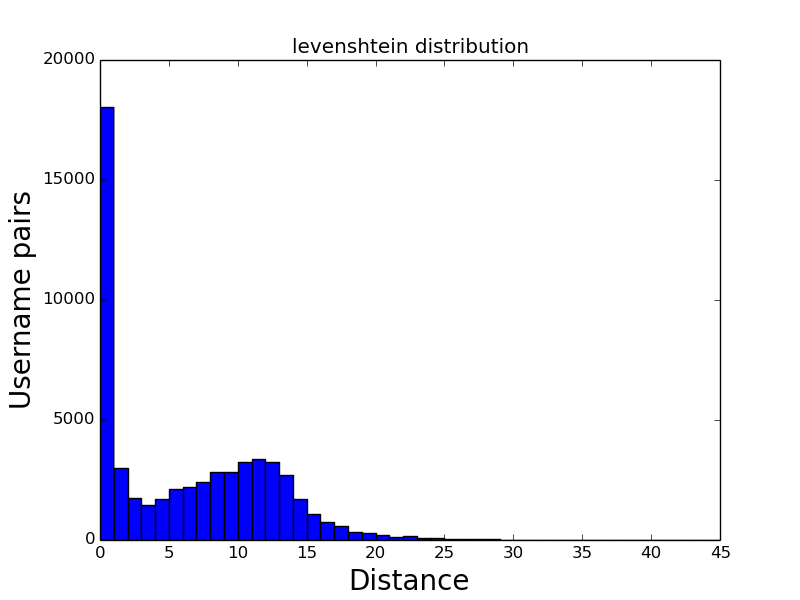
\includegraphics[width=110mm]{chapters/distanceplot/levenshtein_distribution.png}
\caption{Distribuzione della distanza di Levensthein tra coppie di usernames  \label{overflow}}
\end{figure}

\begin{figure}[h!]
\centering
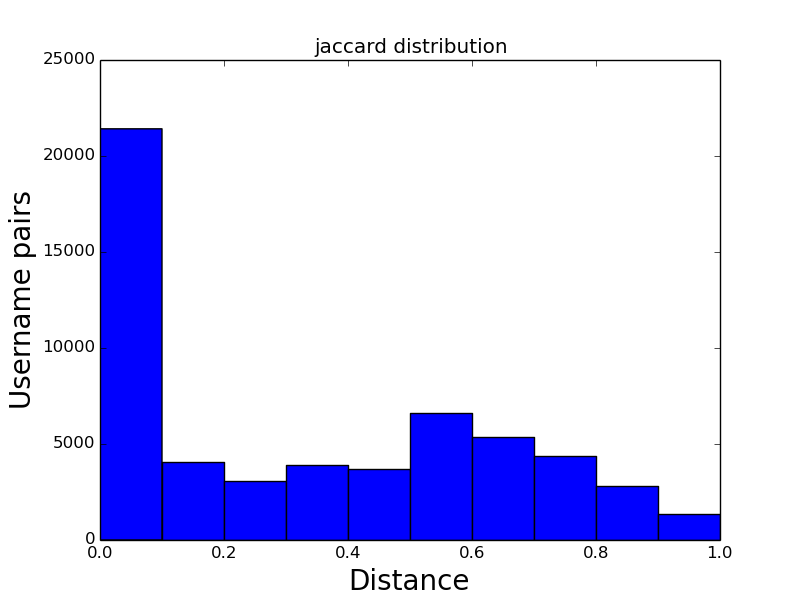
\includegraphics[width=110mm]{chapters/distanceplot/jaccard_distribution.png}
\caption{Distribuzione indice di Jaccard tra coppie di usernames \label{overflow}}
\end{figure}

\newpage

In Fig3 mostriamo come i dati riportino un pattern a \textit{doppio picco} sia su dati globali che su alcune classi prese singolarmente.


\begin{figure}
\begin{subfigure}{.5\textwidth}
  \centering
  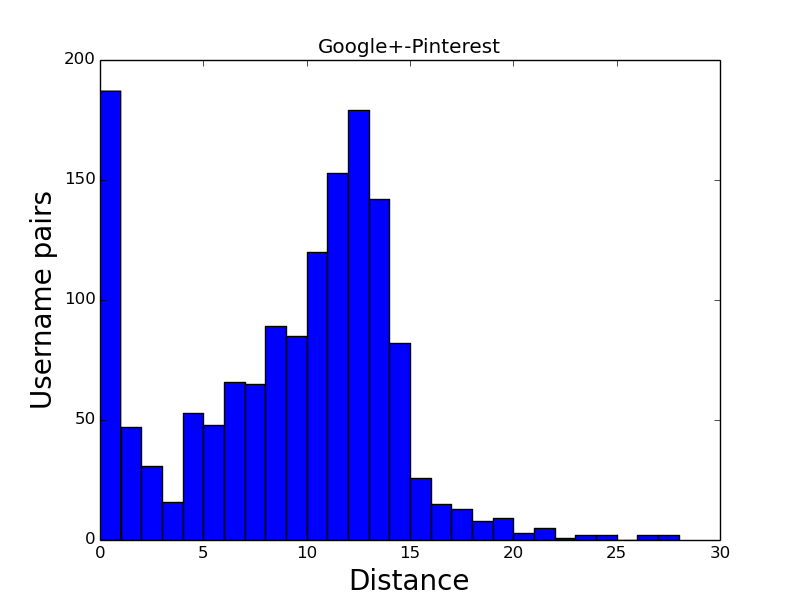
\includegraphics[width=.8\linewidth]{chapters/distanceplot/Google+-Pinterest.png}
  \caption{Google+ Pinterest}
  \label{fig:sfig1}
\end{subfigure}%
\begin{subfigure}{.5\textwidth}
  \centering
  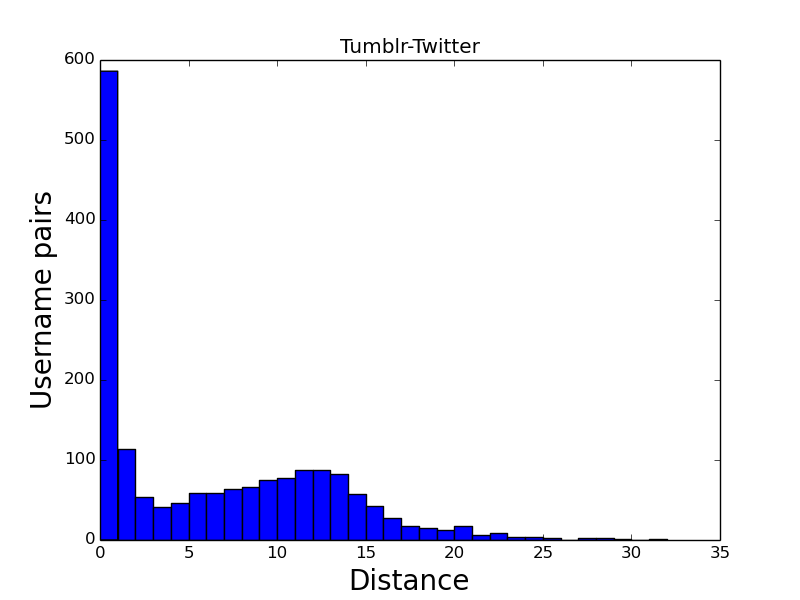
\includegraphics[width=.8\linewidth]{chapters/distanceplot/Tumblr-Twitter.png}
  \caption{Tumblr Twitter}
  \label{fig:sfig2}
\end{subfigure}
\caption{Distribuzione multimodale, con pattern a doppio picco, anche su classe singola}
\label{fig:fig}
\end{figure}

In Fig4 e Fig5 riportiamo la distribuzione delle distanze tra coppie di username casuali, non appartenenti alla stessa persona. Il mescolamento delle coppie di username è ottenuto tramite una tecnica usualmente riferita come \textit{convolution} o \textit{zip function}, una funzione che mappa una tupla di sequenze in una sequenza di tuple. Se ad esempio si ha una lista di 3 coppie/tuple di username \textit{u} per utenti \textit{i}:

\begin{gather*}
  [(i\textsubscript{1}u\textsubscript{1},i\textsubscript{1}u\textsubscript{2}), (i\textsubscript{2}u\textsubscript{1},i\textsubscript{2}u\textsubscript{2}), (i\textsubscript{3}u\textsubscript{1},i\textsubscript{3}u\textsubscript{2})]
\end{gather*}

otteniamo, tramite l'inverso della funzione descritta prima (\textit{unzip}), una lista con due tuple:

\begin{gather*}
  [(i\textsubscript{1}u\textsubscript{1},i\textsubscript{2}u\textsubscript{1}, i\textsubscript{3}u\textsubscript{1}),(i\textsubscript{1}u\textsubscript{2}, i\textsubscript{2}u\textsubscript{2},i\textsubscript{3}u\textsubscript{2})]
\end{gather*}

A questo punto, mescoliamo in maniera casuale l'ordine degli elementi nelle due tuple, e attraverso la funzione zip ricombiniamo le due tuple, ottenendo cosi coppie di username non appartenenti allo stesso utente individuo \textit{i}. Ad esempio potremmo ritrovare:

\begin{gather*}
  [(i\textsubscript{1}u\textsubscript{1},i\textsubscript{2}u\textsubscript{2}), (i\textsubscript{2}u\textsubscript{1},i\textsubscript{3}u\textsubscript{2}), (i\textsubscript{3}u\textsubscript{1},i\textsubscript{1}u\textsubscript{2})]
\end{gather*}


Applichiamo questa tecnica alle coppie di username del nostro dataset, e calcoliamo la distribuzione delle distanze in maniera analoga a quella presentata precedentemente. Quello che riscontriamo è, una piú prevedibile, distribuzione normale (Gaussiana), come si può notare in figure 4 e 5.

\begin{figure}[bp!]
\centering
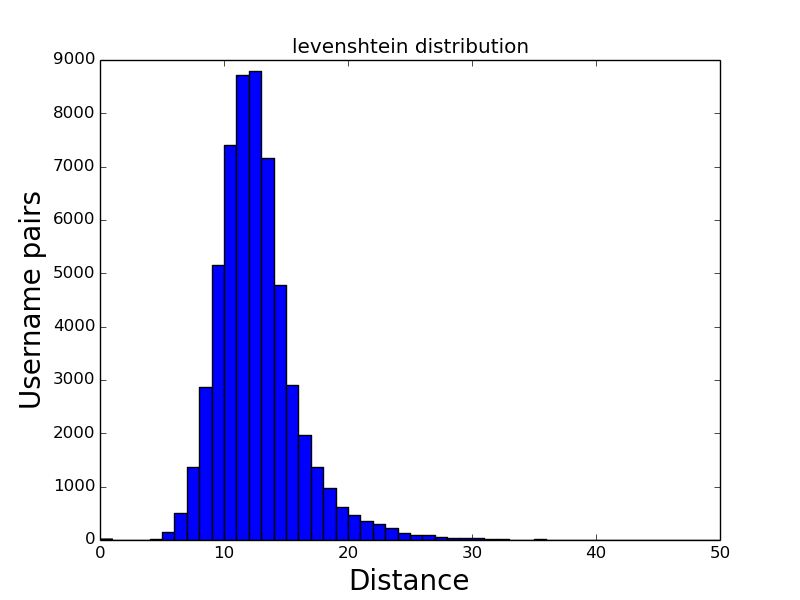
\includegraphics[width=110mm]{chapters/distanceplot/random_levenshtein_distribution.png}
\caption{Distribuzione unimodale distanza di Levensthein tra coppie random  \label{overflow}}
\end{figure}

\begin{figure}[bp!]
\centering
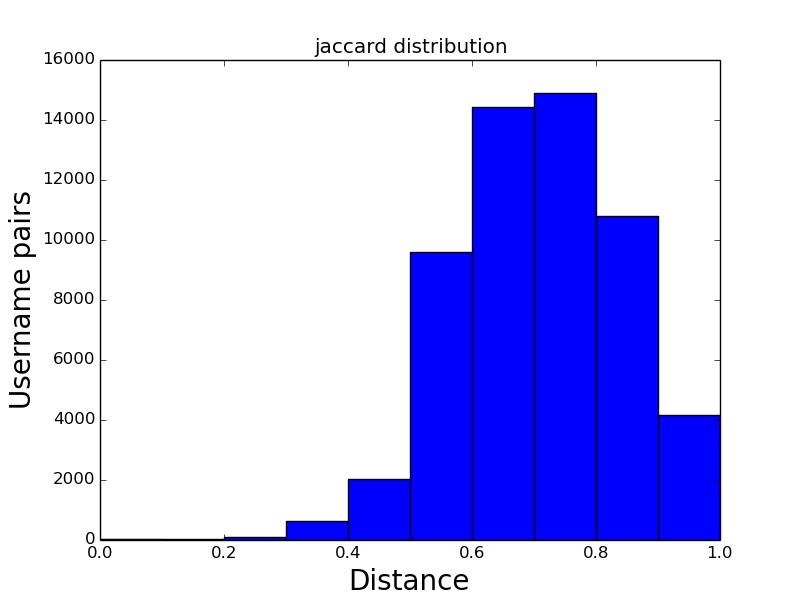
\includegraphics[width=110mm]{chapters/distanceplot/random_jaccard_distribution.png}
\caption{Distribuzione indice di Jaccard tra coppie random \label{overflow}}
\end{figure}
